\section{FSM Flow Chart}
\label{group____fsm__flow}\index{FSM Flow Chart@{FSM Flow Chart}}
This flow chart shows how the FSM works.  




Collaboration diagram for FSM Flow Chart:\nopagebreak
\begin{figure}[H]
\begin{center}
\leavevmode
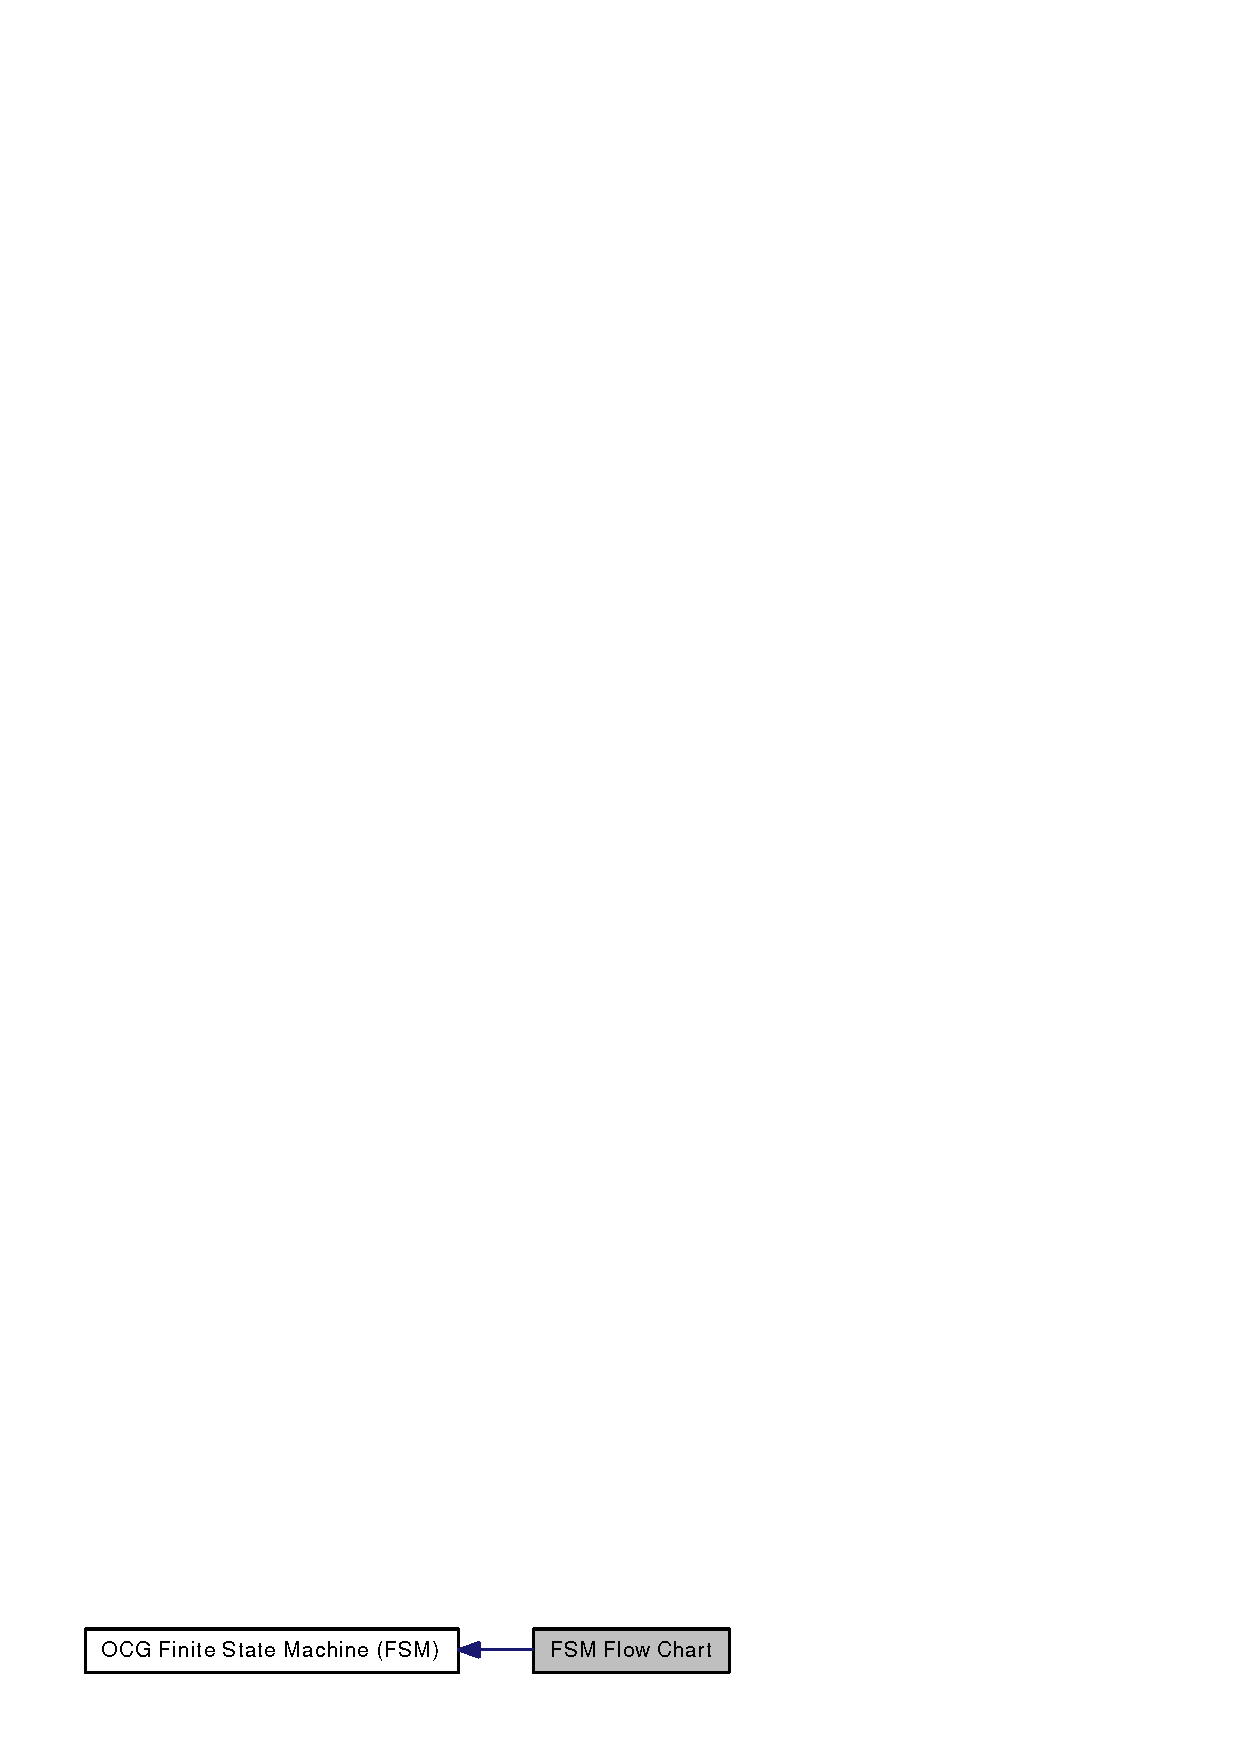
\includegraphics[width=177pt]{group____fsm__flow}
\end{center}
\end{figure}
This flow chart shows how the FSM works. 

There are the following steps the OCG module should contain :\begin{itemize}
\item start OCG\item get option\item detect file\item initiate an emulation\item parse filename\item create directory\item parse XML\item save XML\item call OAI emulator\item generate report\item end OCG\end{itemize}


The following diagram is based on graphviz ({\tt http://www.graphviz.org/}), you need to install the package to view the diagram.

\begin{center}
\begin{ImageNoCaption}\mbox{\includegraphics{inline_dotgraph_1}}
\end{ImageNoCaption}
\end{center}
 